\documentclass{beamer}
\usetheme{Madrid}
\usecolortheme{beaver}
\usepackage{graphicx}
\usepackage{booktabs}
%-------------------------------------------------
\author{Vyshak Puthusseri} 
\date{23th Oct 2019}
\institute[CET]
{
College of Engineering, Trivandrum\\\\
\text{TVE17MCA054 }\\
}

\title{STYLE GAN : A Style Based Generator Architecture for Generative Adversarial Networks}
%-------------------------------------------------



\setbeamertemplate{footline}
{
  \leavevmode%
  \hbox{%
  \begin{beamercolorbox}[wd=.5\paperwidth,ht=2.25ex,dp=1ex,center]{author in head/foot}%
    \usebeamerfont{author in head/foot}\insertshortauthor
    
  \end{beamercolorbox}%
  \begin{beamercolorbox}[wd=.5\paperwidth,ht=2.25ex,dp=1ex,center]{title in head/foot}%

    \insertframenumber{} / \inserttotalframenumber\hspace*{1ex}
  \end{beamercolorbox}}%
  \vskip0pt%
}


\begin{document}
\titlepage 
\begin{frame}
    {Introduction}
    \tableofcontents   
\end{frame}

\section{Deep Learning}
\section{Style Transfer}
\section{GAN : Generative Adversarial Network}
\section{Style Based Generator Architecture for GAN}

\chapter{Deep Learning}
\par
    Deep learning is an artificial intelligence function that imitates the workings of the human brain in processing data and creating patterns for use in decision making. Deep learning is a subset of machine learning in artificial intelligence (AI) that has networks capable of learning unsupervised from data that is unstructured or unlabeled. Also known as deep neural learning or deep neural network. The basic building block of a neural network is known as LTU(Linear Threshold Unit). LTU was only a concept. There will be no learning rule for an LTU. If we apply a learning rule to the architecture it is known as perceptron. It will have a step activation function. SO only binary classifica

%%%%%%%%%%%%%%%%%%%%%%                                          About Style Transfer
\begin{frame}[fragile]{Neural Style Transfer}
   Style transfer relies on separating the content and style of an image. 
   \\
   Given one content image and one style image, we aim to create a new, target image which should contain our desired content and style components:
    \begin{itemize}
        \item feature reconstruction
        \item texture synthesis
    \end{itemize}

\end{frame}


%%%%%%%%%%%%%%%%%%%%%%                                         
\begin{frame}[fragile]{Neural Style Transfer}
    \begin{equation}
        content.image + style.image =  new.image with style.transfered
    \end{equation}
    \begin{figure}[ht]
      \hspace*{-1cm}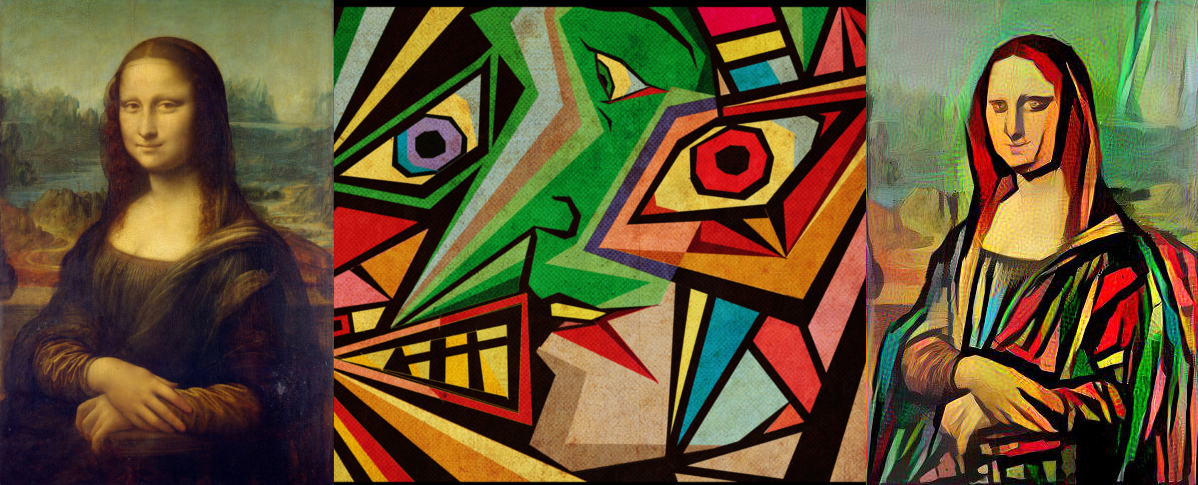
\includegraphics[width=0.5\linewidth]{styletransfer} \\
      \hspace*{-1cm}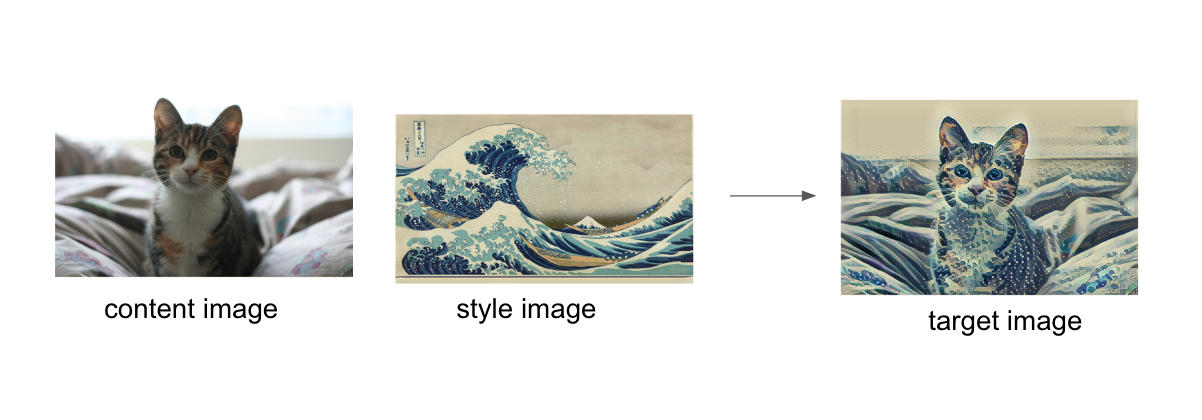
\includegraphics[width=0.7\linewidth]{styletransfercat} 
    \end{figure}
    https://github.com/puthusseri/styleTransfer.git
\end{frame}


%%%%%%%%%%%%%%%%%%%%%%%%%%%%%%%%%%%%%%%%%%%%%%%%%%


%%%%%%%%%%%%%%%%%%%%%%                                          About GAN                    
\begin{frame}[fragile]{Generative Adversarial Network}
 GANs are generative models: they create new data instances that resemble your training data. \\
 eg: images that look like photographs of human faces, even though the faces don't belong to any real person.
     \begin{figure}[ht]
      \hspace*{-1cm}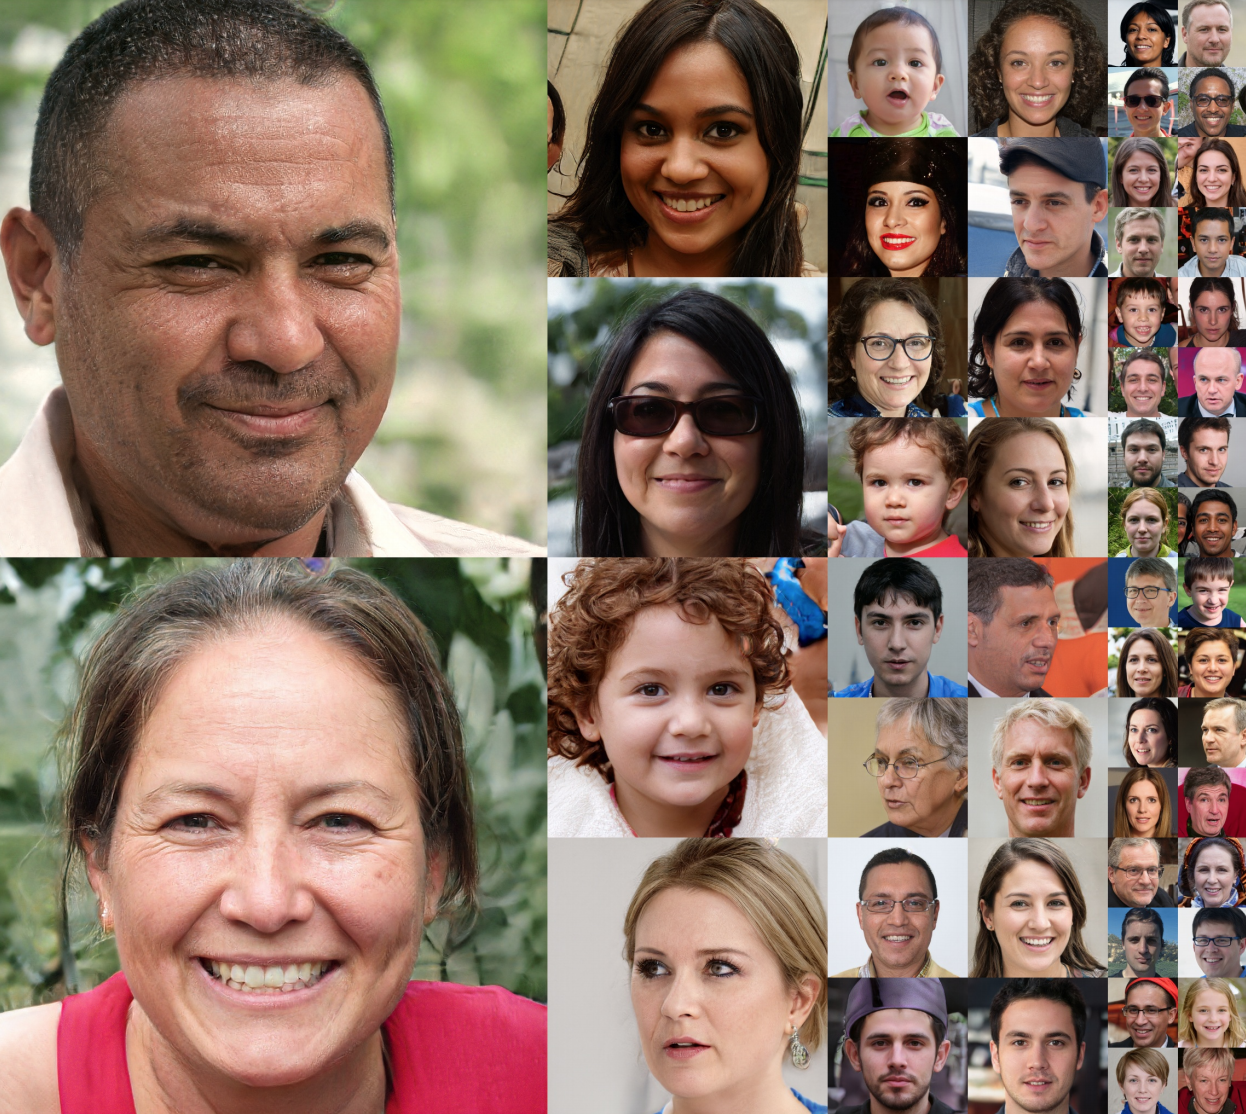
\includegraphics[width=0.5\linewidth]{ganhumans} 

    \end{figure}
\end{frame}

%%%%%%%%%%%%%%%%%%%%%%                                          About GAN Applications                   
\begin{frame}[fragile]{GAN : Applications}

    \begin{itemize}
        \item Image to image translation (in unsupervised way)
        \item blue prints to real image
        \item photo to cartoon (Facebook AI research)
        \item photo of day to night (NVIDIA Research)
        \item Creating stimulated training set (eg : face recognition problem)
        \item for imitaion learning
    \end{itemize}
\end{frame}

%%%%%%%%%%%%%%%%%%%%%%                                          About GAN Overview                   
\begin{frame}[fragile]{GAN : Overview}
 GANs has two parts: \\
    \begin{itemize}
        \item The generator : learns to generate plausible data. The generated instances become negative training examples for the discriminator.

        \item The discriminator: learns to distinguish the generator's fake data from real data. The discriminator penalizes the generator for producing implausible results.
    \end{itemize}
\end{frame}


%%%%%%%%%%%%%%%%%%%%%%                                          About GAN Training                   
\begin{frame}[fragile]{GAN : Training}
     \begin{figure}[ht]
         \hspace*{-1cm}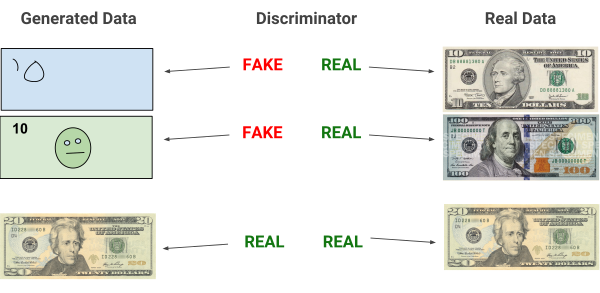
\includegraphics[width=0.7\linewidth]{gantrain} \\ \\ \\ \\ \\ 


    \end{figure}
\end{frame}

%%%%%%%%%%%%%%%%%%%%%%                                          About GAN Architecture                   
\begin{frame}[fragile]{GAN : Architecture}
     \begin{figure}[ht]
         \hspace*{-1cm}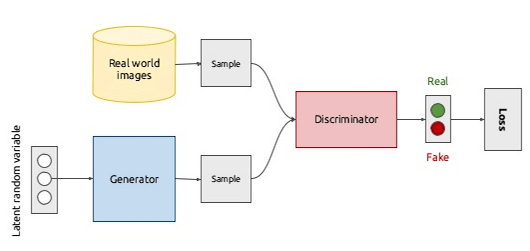
\includegraphics[width=0.7\linewidth]{ganarchitecture.png} \\ \\ \\ \\ \\ 
    \end{figure}
\end{frame}
%%%%%%%%%%%%%%%%%%%%%%%%%%%%%%%%%%%%%%%%%%%%%%%%%%%%%%%%%%%%%%%%%%%%%%

%%%%%%%%%%%%%%%%%%%%%%                                          About Style Based GAN                   
\begin{frame}[fragile]{Style Based GAN}
        \begin{itemize}
        \item Introduced by NVIDIA 
        \item Improved the efficiency of GAN by improving the generator
        \item Introduced new automated metrics - perceptual path length and linear seperability
        \item Result was  : new dataset Flickr Face HQ (FFHQ) of size 2.56 TB
    \end{itemize}

\end{frame}

%%%%%%%%%%%%%%%%%%%%%%                                          About Style Based Generator                   
\begin{frame}[fragile]{Style Based Generator}
        \begin{itemize}
        \item The weights are studied through the 8 layer affine transformation.
        \item Feature maps are normalized using AdaIN
        \item Generate \textit{stochastic details} by introducing the explicit noise for each layer.
        \item Final resulting feature maps are passed to the discriminator.
    \end{itemize}

\end{frame}

%%%%%%%%%%%%%%%%%%%%%%                           About Style Based Generator Architecture                   
\begin{frame}[fragile]{Style Based Generator : Architecture}
     \begin{figure}[ht]
         \hspace*{-1cm}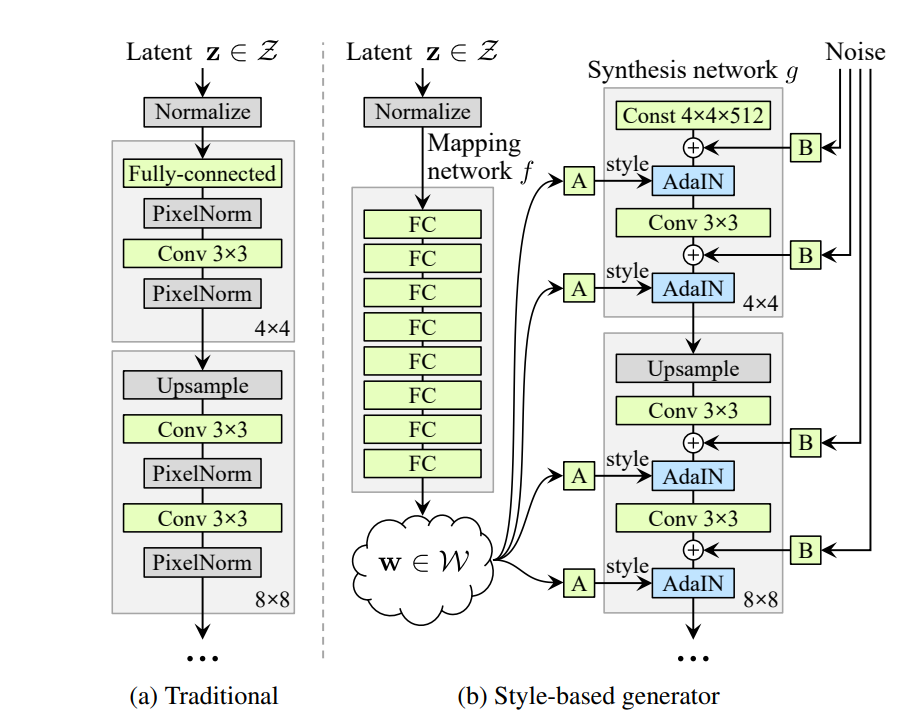
\includegraphics[width=0.9\linewidth]{styleganarchitecture.png} \\ \\ \\ \\ \\
    \end{figure}
\end{frame}

%%%%%%%%%%%%%%%%%%%%%%                                          About Style Based Image Quality                   
\begin{frame}[fragile]{Image Quality }
        \begin{itemize}
        \item Comparing with CelebA-HQ with FFHQ based on Frechet inception distances (FID) , a great improvement happens
        \item Used truncation trick
        \item Used 26.3M parameters for training
        \item Generated image is of 1024 * 1024 resolution
    \end{itemize}

\end{frame}

%%%%%%%%%%%%%%%%%%%%%%%%%%%%%%%%%%%%%%%%%%%%%%%%%%%%%%%%%%%%%%%%%%%%%%

%%%%%%%%%%%%%%%%%%%%%%                                  About Style Based generator Properties  1                 
\begin{frame}[fragile]{Style Based Generator : Properties }
        \begin{itemize}
        \item Style mixing - mixing regularization
    \end{itemize}
    \begin{figure}[ht]
         \hspace*{-1cm}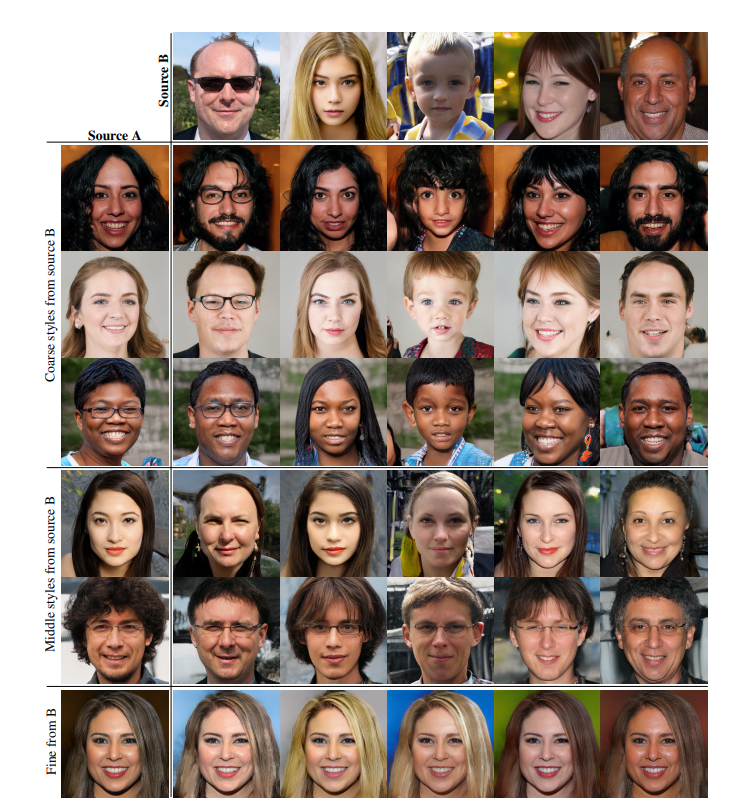
\includegraphics[width=0.6\linewidth]{stylemixing.png} \\ \\ \\ \\ \\
    \end{figure}

\end{frame}

%%%%%%%%%%%%%%%%%%%%%%                                  About Style Based generator Properties  2                
\begin{frame}[fragile]{Style Based Generator : Properties }
        \begin{itemize}
        \item Stochastic variation
    \end{itemize}
    \begin{figure}[ht]
         \hspace*{-1cm}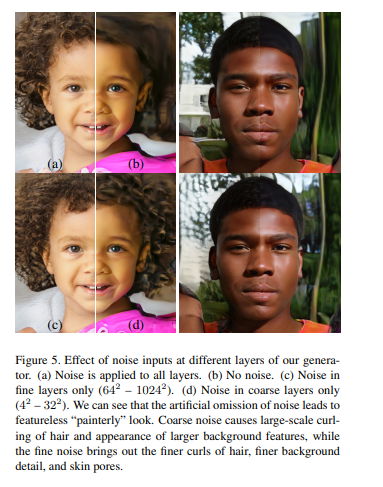
\includegraphics[width=0.7\linewidth]{stochasticvariation.png} \\ \\ \\ \\ \\
    \end{figure}

\end{frame}

%%%%%%%%%%%%%%%%%%%%%%%%%%%%%%%%%%%%%%%%%%%%%%%%%%%%%%%%%%%%%%%%%%%%%%


\section{Conclusion}
\begin{frame}{Conclusion}
    \begin{itemize}
        \item Reduced time complexity of the GAN 
        \item FFHQ image database
        \item Relevance and future scope
    
    \end{itemize}
\end{frame}
\begin{frame}%%     1
\begin{center}
\Huge Thank You!
\end{center}
\end{frame}
%---------------------------------------------------------------
\end{document}